%% apps.tex
%% $Id: apps.tex 61 2012-05-03 13:58:03Z bless $
%%

\chapter{Auswahl der Applikationen}
\label{ch:Apps}
%% ==============================

Die Self-Tracking Apps stellen Optionen zur Verfügung, um einzelne oder mehrere Messdaten manuell oder automatisch zu erfassen. 
Die meisten Apps beschränken sich dabei auf bestimmte Self-Tracking-Aktivitäten, z.B. nur die Erfassung des Ortes, der Stimmung oder der Arbeitszeiten, andere versuchen umfassende Datensammlungen zu realisieren und in Relation zu setzen, z.B. LifeMash \cite{web:SleepCycle}. \\
Für den Gesundheitsbereich beziffert Rauner in seinem Artikel „Das Handy als Hausarzt“ über 15.000 Gesundheits-App, die aktuell auf dem Markt verfügbar sind. 
Viele der Apps bieten die Möglichkeit die gesammelten Messwerte über das Internet im dazugehörigen jeweiligen eigenen Internetprofil zu speichern oder bestimmte Daten über soziale Netzwerke mit Freunden zu teilen. 
Bekannte Beispiele sind hier z.B. die auf Echtzeit-GPS-Lokalisierungen basierenden Fitnesstracker Endomondo und RunKeeper, die sich mit dem Facebookaccount verknüpfen lassen. 
\\
\\
Zur Durchführung und Erhebung der Daten wurden drei verschiedene mobile Anwendungen von der Projektgruppe ausgesucht und festgelegt.
Zum Tracken der Aktivtäten wurde die kostenlose Anwendung Moves ausgewählt, für das Erfassen der Schlafrhythmen die kostenpflichtige Anwendung SleepCycle und für die Erfassung der Stimmung die Anwendung Hueman.
Durch diese Applikationen sind die Hauptbereiche, auf denen das Augenmerk für ein erfolgreiches Durchführen des Projektes liegt, abgedeckt.
Die Apps werden im Folgenden genauer beschrieben.


%% ==============================
\section{Moves}
%% ==============================
\label{ch:Apps:sec:Moves}

\subsection{Was ist Moves?}
%% ==============================
\label{ch:Apps:sec:Moves:subsec:WIM}

Moves ist eine mobile Quantified-Self-Anwendung, die die täglichen Aktivitäten trackt, mit der Hoffnung für den Anwender, durch die gewonnenen Daten besser in Form zu kommen. 
Seit Anfang 2013 ist die Applikation, die ursprünglich nur für iPhone und iPad entwickelt wurde kostenlos in den AppStores erhältlich. 
Die Moves-App wurde mittlerweile mehr als 3,5 Millionen Mal heruntergeladen und erhielt im Jahr 2013 zudem die Auszeichnung als "Best of AppStore 2013".
Seit Anfang 2014 ist die Anwendung nun auch auf Android-Plattformen nutzbar und kann so auch dort das Radfahren, Wandern oder Laufen tracken.

\ref{fig:Haupt-UI}

\begin{figure}[h]
\centering
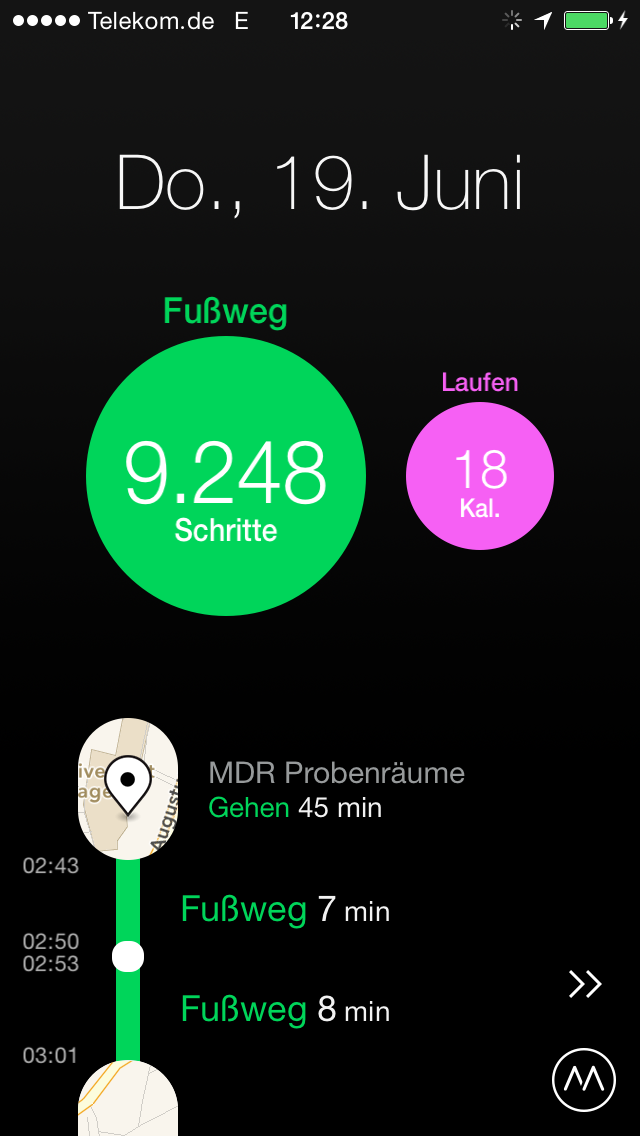
\includegraphics[scale=0.3]{images/moves-app-main-ui.PNG}
\caption{Moves Haupt-UI \cite{fig:Haupt-UI}}
\label{fig:Haupt-UI}
\end{figure}

\subsection{Design und Features}
%% ==============================
\label{ch:Apps:sec:Moves:subsec:DuF}

Moves hebt sich von den mittlerweile massenhaft existierenden Bezahl-Fitness-Apps und diversen tragbaren Geräten, wie zum Beispiel Fitbit One, das Nike Fuelband oder dem Withings Pulse, insofern sehr stark ab, dass die Daten hier in sehr viel benutzerfreundlicher Art und Weise präsentiert werden, als bei den zuvor genannten.
\\
Die App glänzt durch eine gute Umsetzung und ihrer Einfachheit. 
Viele andere Fitness-Apps bombardieren den Nutzer regelrecht mit den bereitgestellten bzw. erfassten Daten, um diesen "ruhig" zu stellen. 
Moves hingegen nimmt einen ganz anderen Ansatz wahr. 
Dem Nutzer werden die Daten, die durch die täglichen Aktivitäten erhalten wurden, als "Handlung" bzw. Timeline des Tages anschaulich präsentiert.
\\
Der Einsatz von Sensoren, wie zum Beispiel dem Beschleunigungsmesser, gepaart mit GPS- und WiFi machen es so der Applikation möglich, zwischen den verschiedenen Aktivitäten des Nutzers, sowie dessen Stadtorte zu unterscheiden. 
Die gewonnenen Daten werden auf den hauseigenen Servern der Firma gespeichert, auf denen unter anderem auch ein Teil der Daten analysiert wird. 
Bei täglicher Nutzung von Moves fallen so etwa 30 MB an Daten an, die auf die Server geschoben werden. 
Das heißt natürlich nicht, dass die Anwendung nur online genutzt werden kann und dadurch das monatliche Übertragungs-Volumen schmälert. 
Eine Volumenschonende Nutzung - also offline - ist möglich, da die App die notwendigen Daten auch so sammelt, diese aber erst analysieren und auswerten kann, wenn wieder eine aktive Verbindung zum Internet, z.B. durch WiFi, besteht.   
\\
Die Benutzeroberfläche an sich ist eher spärlich gehalten. 
Es gibt lediglich die "Storyline" bzw. die Timeline, die herunterscrollbar ist. 
Weiterhin existieren dreierlei Kreistypen, die oberhalb der Timeline angebracht sind und die jeweilige Aktivität, wie Wandern, Radfahren oder Laufen, darstellt. 
Diese zeigen dem Nutzer neben den getätigten "Schritten" auch die Menge an verbrauchten Kalorien und die zurückgelegte Strecke in Kilometern an. 
Weiterhin bietet die die App Moves die Möglichkeiten Fortschritte herauszukristallisieren, da man aktuelle Aktivitäten mit denen vom Vortag oder der Vorwoche vergleichen kann.   
\\
\ref{fig:Timeline}

\begin{figure}[h]
\centering
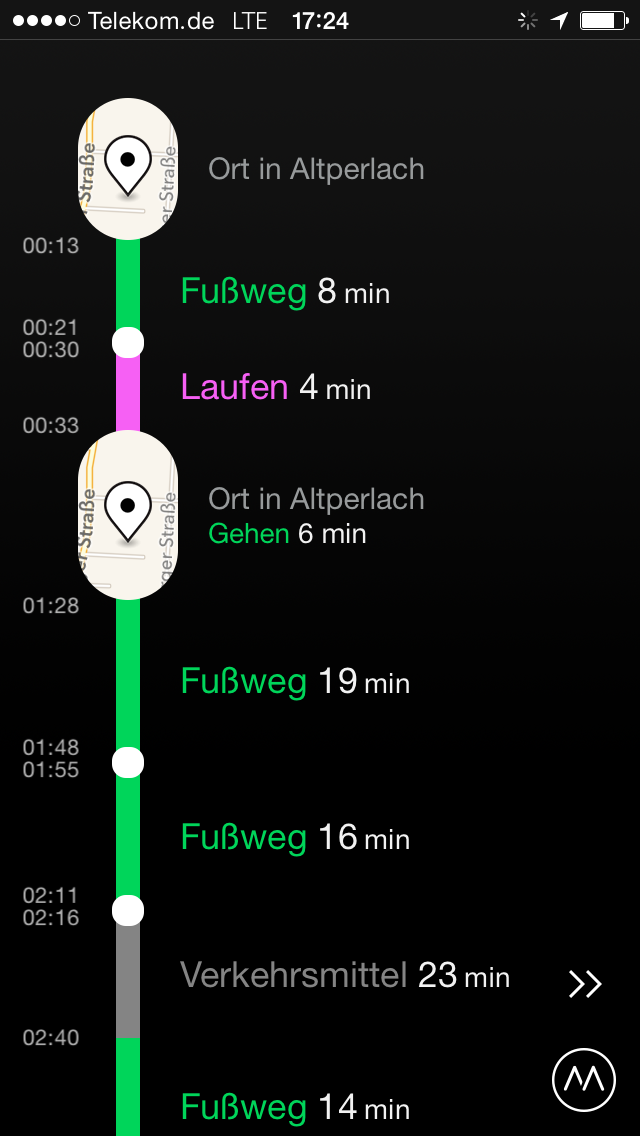
\includegraphics[scale=0.3]{images/moves_app_screenshot.png}
\caption{Moves Timeline \cite{fig:Timeline}}
\label{fig:Timeline}
\end{figure}

Die Einstellungen der Applikation sind ziemlich minimalistisch gehalten, da der Nutzer lediglich die Möglichkeiten hat, die Batterielebensdauer durch die Auswahl des stationären Einsatzes zu minimieren, die Messeinheiten zwischen "metrisch" und "imperial" ändern und einen täglich Aktivitätsbericht als Benachrichtigung erhalten kann. 
\\
Die Einbindung durch sogenannte "Third-Party-Apps", also von Anwendungen anderer Hersteller, ist seit Anfang 2014 möglich und erweitert das Repertoire von Moves enorm. 
So ist die Einbindung von bis zu 13 anderen Apps, wie TicTrac oder Bounts derzeit möglich.  
\\
\ref{fig:Anwendungen}

\begin{figure}[h]
\centering
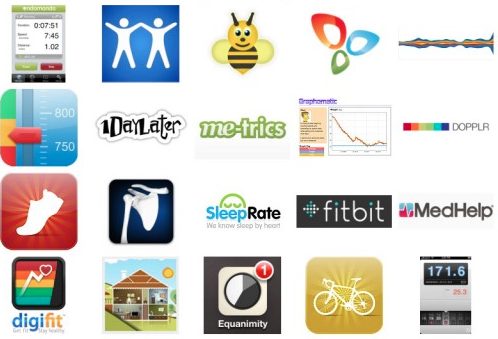
\includegraphics[scale=0.3]{images/qs-anwndungen-gadgets.png}
\caption{Verschiedene QS Anwendungen und Gadgets \cite{fig:Anwendungen}}
\label{fig:Anwendungen}
\end{figure}

\subsection{Die Performance}
%% ==============================
\label{ch:Apps:sec:Moves:subsec:PERF}

Das Großartige an der App Moves ist, dass der Nutzer kein extra Gerät - wie eine "Uhr" am Handgelenk - benötigt, um die Datengenerierung zu ermöglichen, sondern lediglich das Smartphone bzw. Tablet des Nutzers alleine genügt. 
Auch wird durch das "Always-on"-Prinzip, also dass die Anwendung durchgehend im Hintergrund geöffnet ist, die ständige Datengenerierung gewährleistet, auch wenn der Nutzer einmal vergessen sollte, Moves zu öffnen.
\\
Da die Genauigkeit der Daten offensichtlich ein wichtiges Anliegen der Entwickler ist, zeigt sich im Vergleich mit der Tracking-App Withings Pulse, der einen Unterschied von ganzen 200 Schritten zeigte. 
Auch in Hinblick auf die angezeigte Distanz und Dauer war Moves so akkurat wie ein modernes TomTom GPS-Navigationsgerät.
\\
\ref{fig:GPS-Map}

\begin{figure}[h]
	\centering
	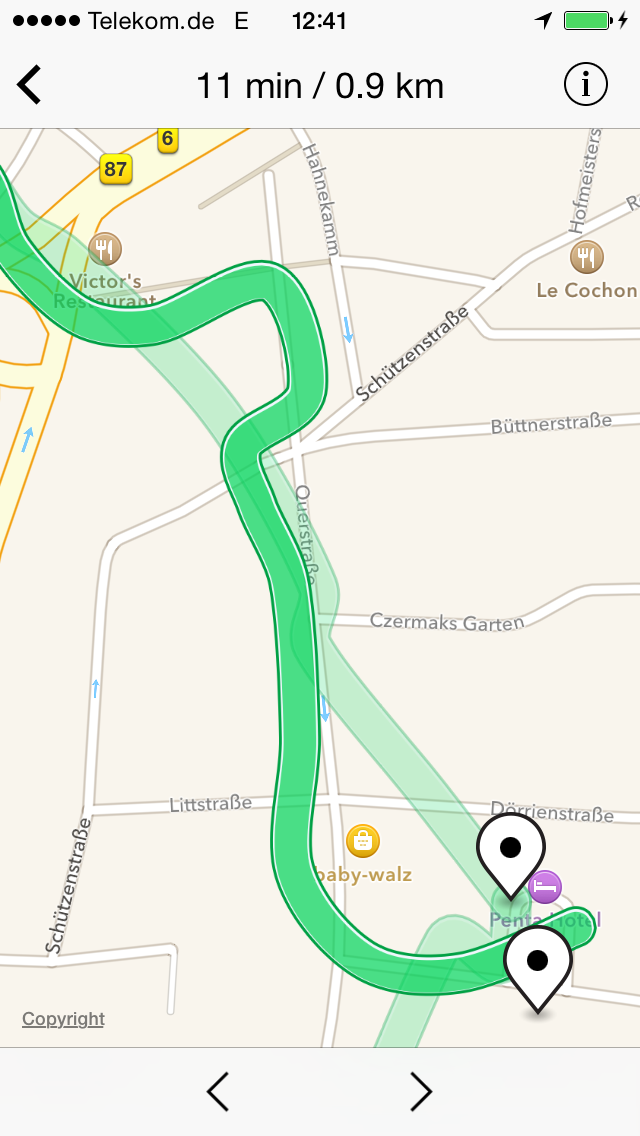
\includegraphics[scale=0.3]{images/moves-app-map.PNG}
	\caption{Moves GPS-Map \cite{fig:GPS-Map}}
	\label{fig:GPS-Map}
\end{figure}

Wie bei den meisten Apps, die sehr stark auf GPS setzen, um reibungslos funktionieren zu können, geht die Moves-Nutzung derweil stark auf die Akkulaufzeit des Smartphones/Tablets, was sich trotz verbesserter Technologie im Zusammenhang mit dem M7-Chip des iPhone 5S sehr bemerkbar macht. 
So raten die Entwickler den Nutzern, das Smartphone/Tablet immer über Nacht aufladen zu lassen bzw. den stationären Einsatz einzustellen.
\\
Der normalen täglichen Nutzung der App tut die etwas verkürzte Akkulaufzeit aber kein Abbruch. 
Man sollte lediglich darauf achten, andere Anwendungen stets zu schließen.

\subsection{Zusammenfassung}
%% ==============================
\label{ch:Apps:sec:Moves:subsec:VERDICT} 

Die Moves-App wird den Nutzer vielleicht nicht sofort fitter machen, das ist ja auch nicht die grundlegende Idee hinter der App. 
Es geht vielmehr darum, dem Nutzer ein "gesünderes" Denken durch die Nutzung der Anwendung mit auf den Weg zu geben. 
So kann sich der Nutzer erstmal ein klareres Bild seiner Tagesaktivitäten und Bewegungen machen und so in die Lage versetzt werden, etwas an seinen Aktivitäten zu ändern bzw. zu verbessern.
\\
So eignet sich die App Moves trotz der kleinen Macken, wie Innennutzung oder Akkulaufzeit, sehr gut um mit einer gesünderen veränderten Aktivitätsplanung ins weitere Leben zu starten und schont zugleich den Geldbeutel, da der Nutzer auf die Anschaffung eines teuren Fitness-Tracking-Geräts verzichten kann.

%% ==============================
\section{Hueman}
%% ==============================
\label{ch:Apps:sec:Hueman}

\subsection{Was ist Hueman?}
%% ==============================
\label{ch:Apps:sec:Hueman:subsec:WIH}

Human ist eine weitere mobile QS-Anwendung, mit der sich das allgemeine tägliche Befinden tracken lässt. 
Durch die dadurch gewonnen Daten soll der Nutzer etwaige positive oder negative Veränderungen durch bestimmte Aktivitäten erkennen und besser einordnen.
Seit Anfang 2014 ist die Applikation in Apples' AppsStore erhältlich, um die Gemütszustände zu erfassen.


\subsection{Design und Features}
%% ==============================
\label{ch:Apps:sec:Hueman:subsec:DuFe}

Auch die Entwickler dieser Anwendung schreiben das Wort "simplicity" groß. 
Denn durch einfaches Wischen des Nutzers über den Bildschirm des Smartphones legt dieser seinen aktuellen Gefühlszustand fest.
\ref{fig:HUI}

\begin{figure}[H]
	\centering
	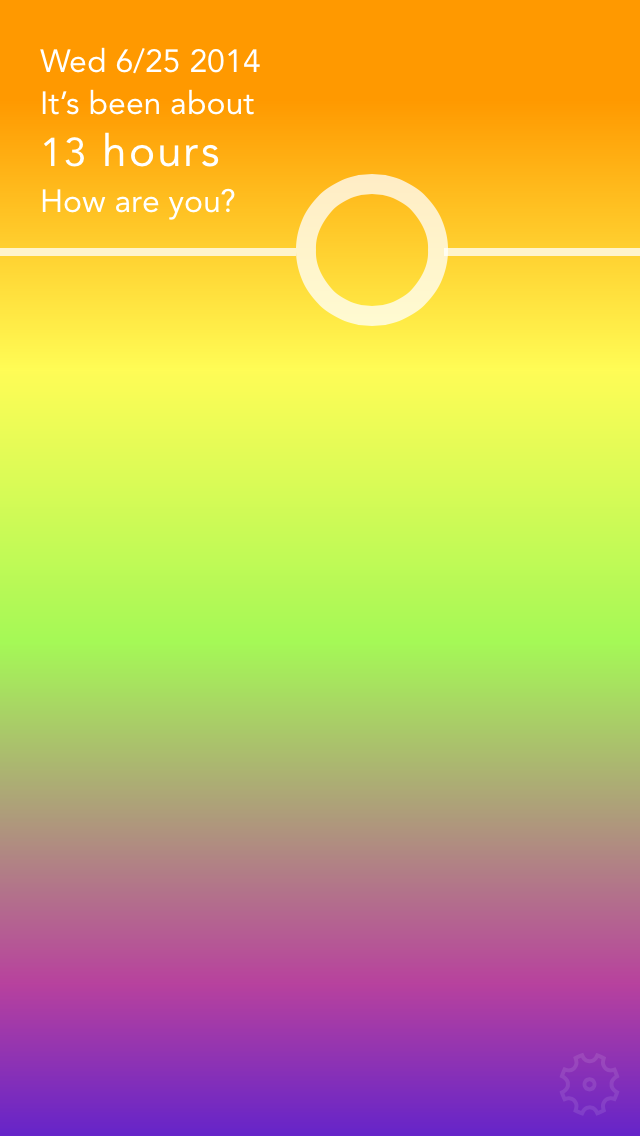
\includegraphics[scale=0.3]{images/hueman-app-main-ui.PNG}
	\caption{Hueman UI \cite{fig:HUI}}
	\label{fig:HUI}
\end{figure}

Optisch aufgewertet werden die einzelnen Zustande durch eine Art Farbpalette, bei der die "waren" Farben für eine gute bis sehr gute und die "kalten" Farben für die schlechte bis miserable Stimmung stehen.
Die Applikation vergleicht die einzelnen gewonnenen Daten miteinander und gibt diese dem Nutzer als fortlaufendes Diagramm aus, sodass er die Veränderungen der Stimmungen schnell erkennen kann.
\ref{fig:Vergleich}

\begin{figure}[H]
\centering
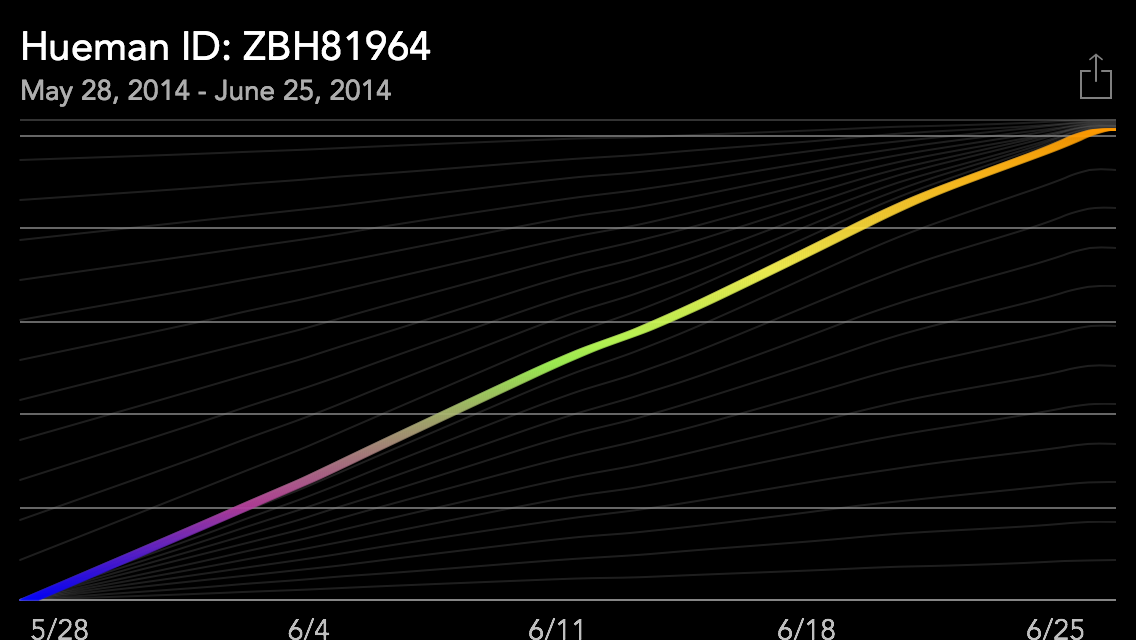
\includegraphics[scale=0.3]{images/hueman-matched-data.PNG}
\caption{Hueman Vergleich \cite{fig:Vergleich}}
\label{fig:Vergleich}
\end{figure}


\subsection{Zusammenfassung}
%% ==============================
\label{ch:Apps:sec:Hueman:subsec:Verdict}

Da sich die App Hueman leicht und vor allem schnell bedienen lässt, ist sie der optimale Begleiter für Nutzer, die gerne mehr über die Wechselwirkungen ihrer Stimmung Bescheid wissen wollen.
Sie erlaubt es durch einfache grafische Aufwertungen, dem Nutzer auch visuell seine Stimmungen näher zubringen.  


%% ==============================
\section{Sleep Cycle}
%% ==============================
\label{ch:Apps:sec:SleepCycle}

Sleep Cycle ist ein Schlafphasenwecker, welcher das Schlafmuster des Benutzers analysiert und in der leichtesten Phase des Schlafes aufweckt. \cite{web:SleepCycle}
Dafür zeichnet die Software die Bewegungsaktivitäten während des Schlafes auf und wertet diese aus.
Darüber hinaus biete die Applikation zusätzliche Möglichkeiten um die Schlafgewohnheiten zu Kategorisieren sowie die Auswirkungen in unterschiedliche Charts zu begutachten. 
Die Idee von intelligenten Schlafphasenweckern besteht darin, die Schlafgewohnheit aufzuzeichnen und mit Notizen zu versehen. Dadurch erlangt man die Erkenntnis über die Schlafqualität in Zusammenhang mit deren Ursachen, um im Anschluss die eignen Gewohnheiten zu verändern, damit die Qualität des Schlafes zu verbessern und sich erholter zu fühlen.

\subsection{Hintergrundwissen}
\label{ch:Apps:sec:Sleepcycle:subsec:H}

Der Schlaf ist ein wichtiges aktiver Teiles des täglichen Lebens und dient der Erholung von Körper und Geist.
Bei zu wenig Schlaf leidet der Körper unter Schlafmangel und kann zu Depressionen, Bluthochdruck oder weiteren Krankheiten führen. \cite{Chen:SleepMonitoring}

Das bereits ca. 15\% der Bevölkerung in Deutschland an immer wiederkehrenden Schlafstörungen leiden und dem Steigenden Interesse an \textbf{Quantified Self \ref{ch:Grundlagen:sec:QuantifiedSelf}}, sind Gründe für immer mehr der sogenannten "Sleep Tracker" auf dem Markt. %\cite{•}
Mit diesen, als reiner Software auf dem Smartphone (Bsp. \textbf{Sleep Cycle \ref{ch:Apps:sec:SleepCycle}}) oder mit zusätzlicher Hardware (Bsp. JawboneUp), lässt sich der Schlaf des Benutzers analysieren und eventuelle Schwachstellen aufzeigen.

Praktisch bewegt sich der Mensch in den verschieden Phasen des Schlafes unterschiedlich stark.
Diese einzelnen Bewegungen zeichnet die Software „Sleep Cycle“ mit Hilfe des eingebauten „Accelerometer“ (dt. Beschleunigungssensor) des Aufzeichnungsgerätes (Smartphone) auf.
Der Schlaf wird generell in folgende 5 Stadien untergliedert:

\begin{itemize}
	\item Einschlafphase (1 Phase)
	\item Leichter Schlaf (2 Phase)
	\item Mittlerer Schlaf (3 Phase)
	\item Tiefer Schlaf (4 Phase)
	\item REM Schlaf (5 Phase)
\end{itemize}

Von Phase eins bis vier nehmen die Bewegungen der Muskel ab, bis diese während des REM Schlafes vollkommen versiegen.
Diese Zyklus dauert circa 90 Minuten und wird während des Schlafes mehrmals durchlaufen.
Dadurch lassen sich die einzelnen Phasen des Schlafes anhand der Bewegung bestimmen. \textbf{BELEGEN}
Innerhalb der ersten beiden Phasen befindet sich der Körper in Momenten in denen er fast Wach ist. Zu diesem Zeitpunkt ist der Benutzer am leichtesten zu Wecken und fühlt sich ausgeschlafener und erholter.
Mit Hilfe der ermittelten Phase und dem gewählten Weckzeitraum, ertönt der Wecker sobald sich der Benutzer in der Leichtesten Phase des Schlafes befindet. Siehe Abbildung \ref{fig:Hypnogramm}


\begin{figure}[H]
\centering
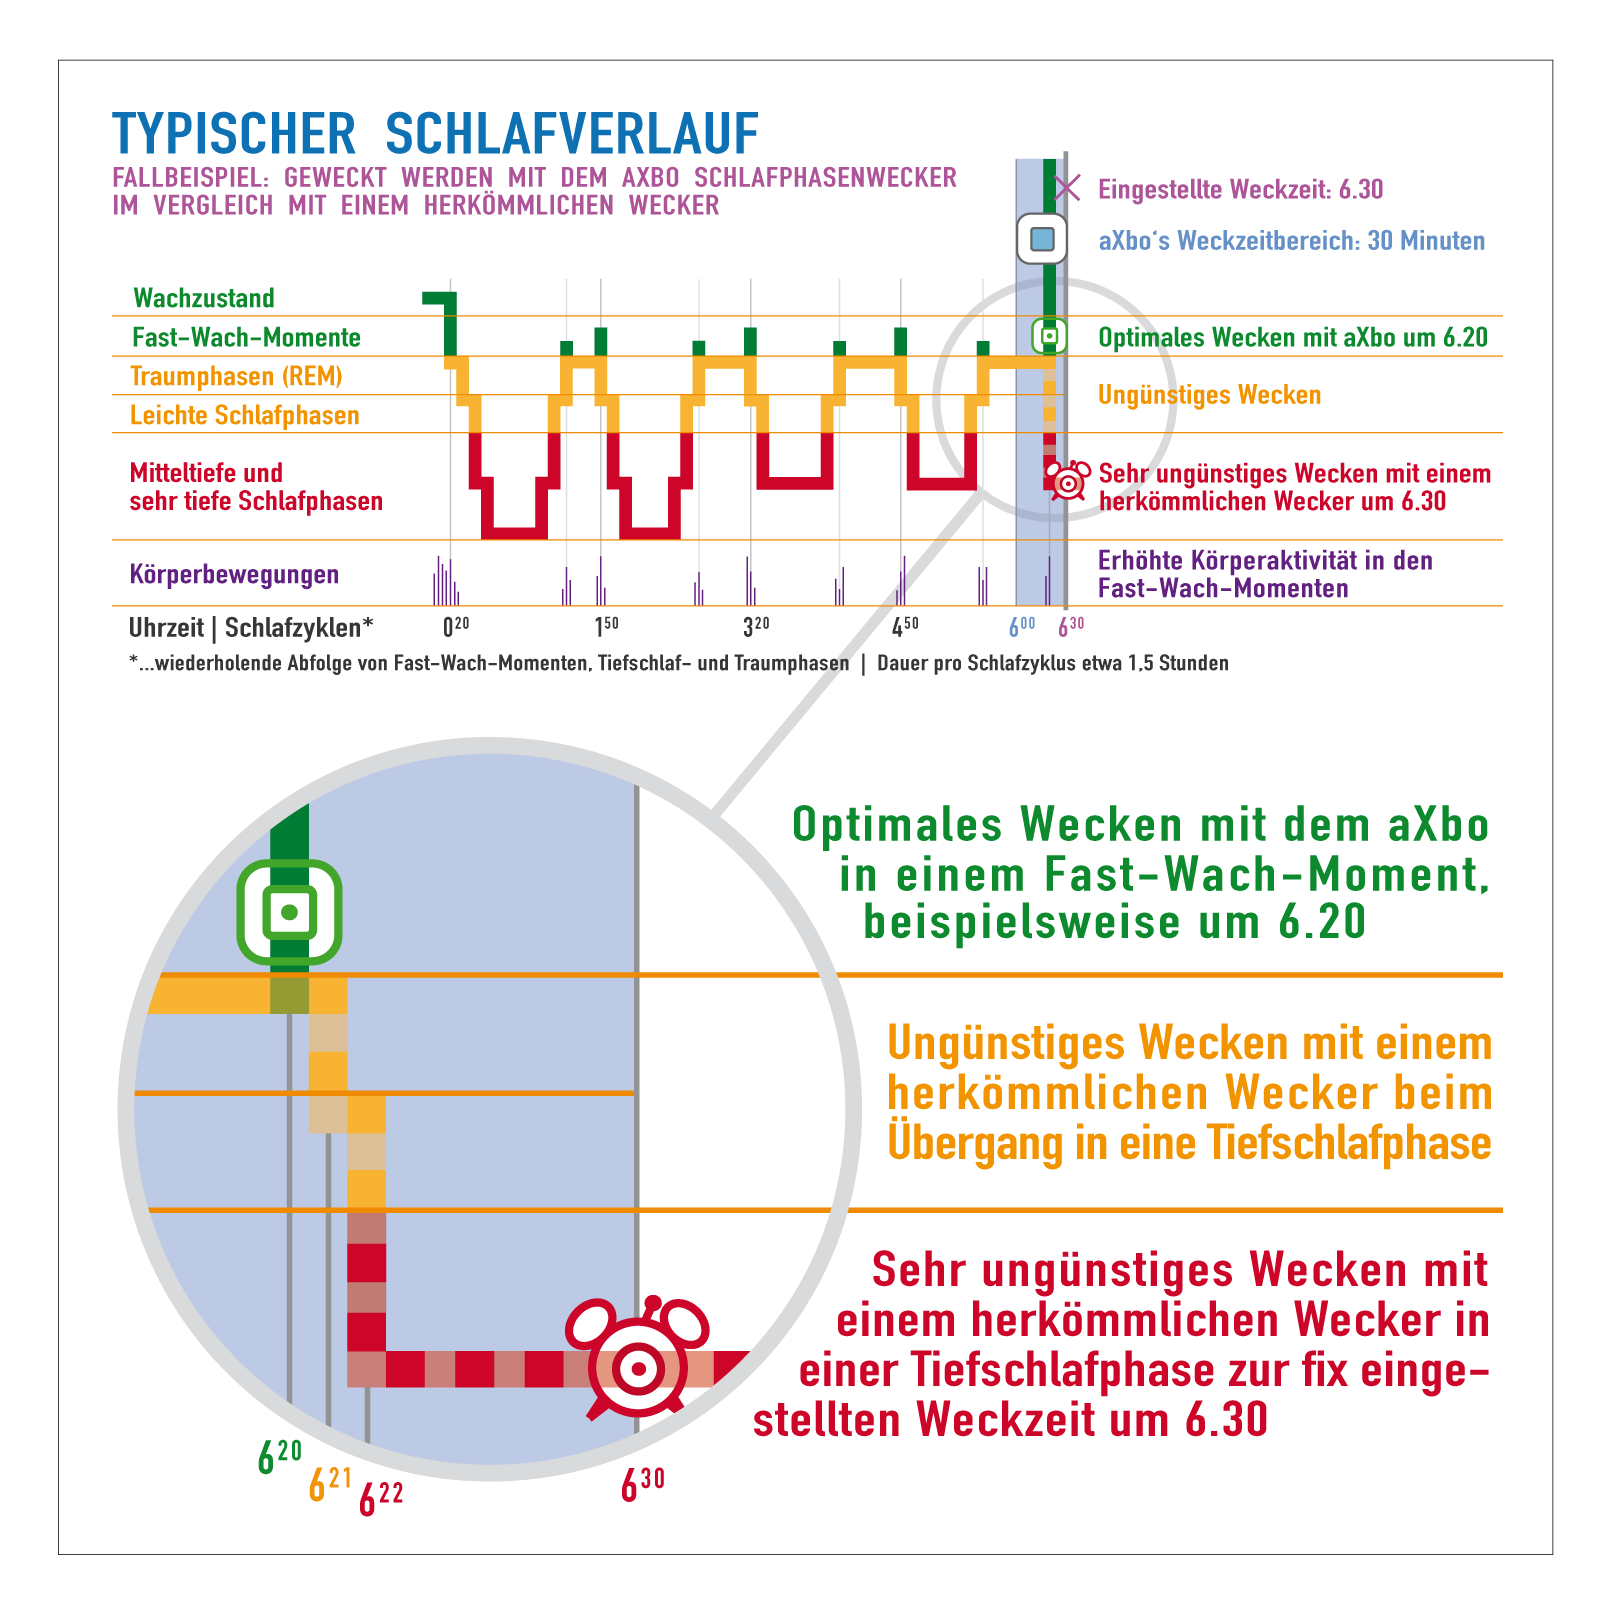
\includegraphics[width=0.9\textwidth]{images/aXbo_Schlafverlauf_Hypnogramm_DE.png}
\caption{Schlafverlauf Hypnogramm \cite{fig:Hypnogramm}}
\label{fig:Hypnogramm}
\end{figure}


\subsection{Funktionsweise und Anwendung}
\label{ch:Apps:sec:Sleepcycle:subsec:FuA}

Um das Ziel eines Schlafphasenweckers zu erreichen, bietet \textbf{Sleep Cycle} mehrere Funktionen und Anwendungsszenarien an.

Zur Initialisierung des Wecker, wird zunächst wie in Abbildung \ref{fig:SCAlarm} gezeigt, die spät möglichste Weckzeit eingestellt.
Außerdem wird das Intervall der Aufwachphase angezeigt.
Die Standardeinstellung für den Weckzeitraum beträgt 30 Minuten.
Eine Konfiguration dieser "`Wake up phase"' lässt sich in den Einstellungen (Abb. \ref{fig:SCSettings}) der App vornehmen.

Nach dem setzen des Weckers erscheint die "`Sleep Note Today"' Ansicht (Abb. \ref{fig:SCSleepNoteToday}), welche der Kategorisierung des Tages vor dem Schlaf dient. Dadurch lassen sich Rückschlüsse auf die täglichen Gewohnheiten schließen und die darauffolgende Schlafqualität beurteilen. \\
Zum Schluss wird das Smartphone neben dem Kopfkissen auf dem Bett platziert.
Aufgrund der dauerhaften Benutzung des Beschleunigungssensor, ist es notwendig das Smartphone während der gesamten Betriebszeit am Netzteil angeschlossen werden.

\begin{figure}[]
  \centering
  \begin{minipage}[b]{0.47\textwidth}
    \centering
    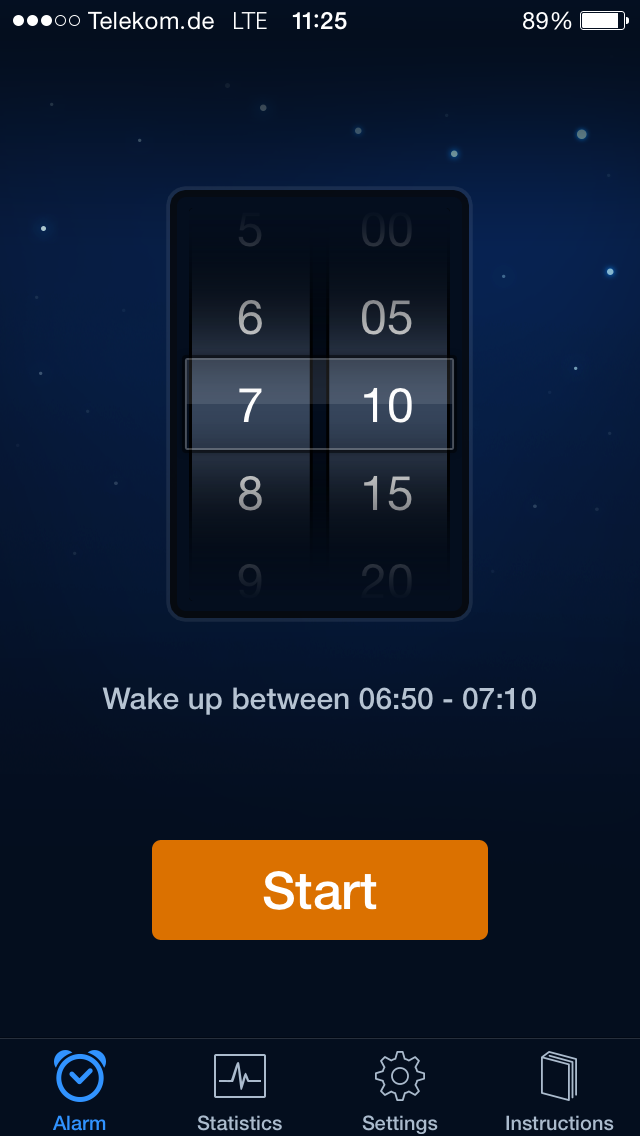
\includegraphics[scale=0.3]{images/SleepCycle/Alarm} 
    \caption{Sleep Cycle Alarm}
    \label{fig:SCAlarm}
  \end{minipage}
  \begin{minipage}[b]{0.47\textwidth}
    \centering
    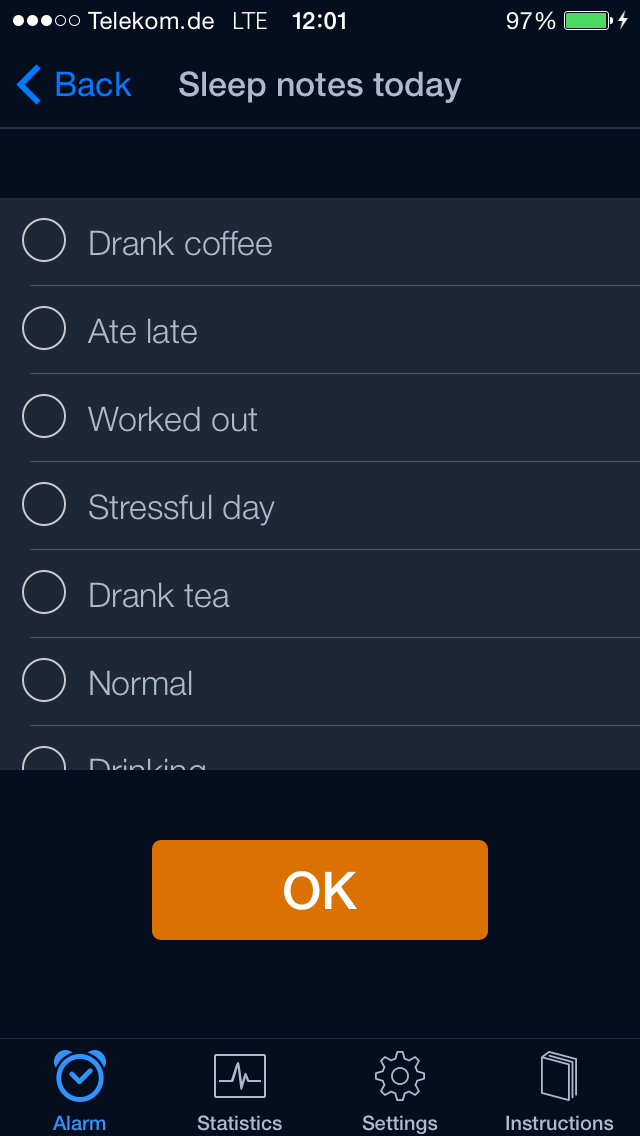
\includegraphics[scale=0.3]{images/SleepCycle/SleepNotesToday}  
    \caption{Sleep Cycle Sleep Note}
    \label{fig:SCSleepNoteToday}
  \end{minipage}
\end{figure}

Zusätzlich bietet \textbf{Sleep Cylce} weitere Einstellungs, Tracking und Analyse Funktionen, die dem Erfolgreichen Auswerten dienen.
In den Einstellung lassen sich unterschiedliche Möglichkeiten des Weckens wählen, sowie zusätzliche Sinnvolle Features aktivieren, mit denen die Analyse vereinfacht werden kann.
Zum einen lässt sich die Stimmung des Benutzer aufnehmen, wie leicht er aufgewacht ist.
Zum anderen kann mit Hilfe der Kamera der Puls des Benutzers ermitteln \cite{web:Pulsmessen}.

\begin{figure}[H]
  \centering
  \begin{minipage}[b]{0.47\textwidth}
    \centering
    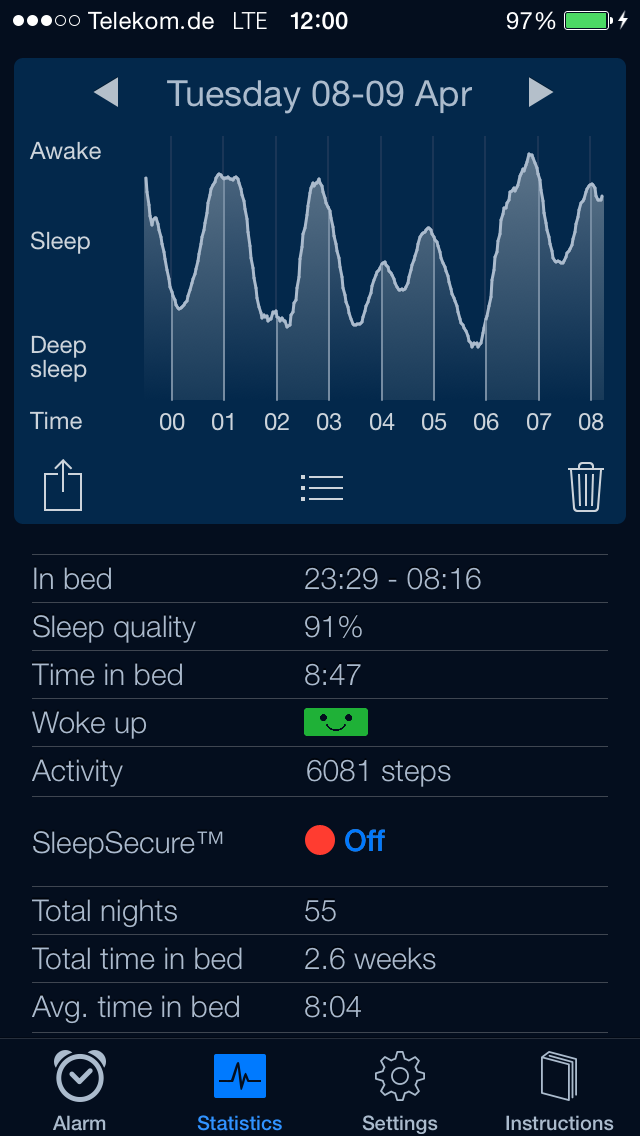
\includegraphics[scale=0.3]{images/SleepCycle/Detail} 
    \caption{Sleep Cycle Detail}
    \label{fig:SCDetail}
  \end{minipage}
  \begin{minipage}[b]{0.47\textwidth}
    \centering
    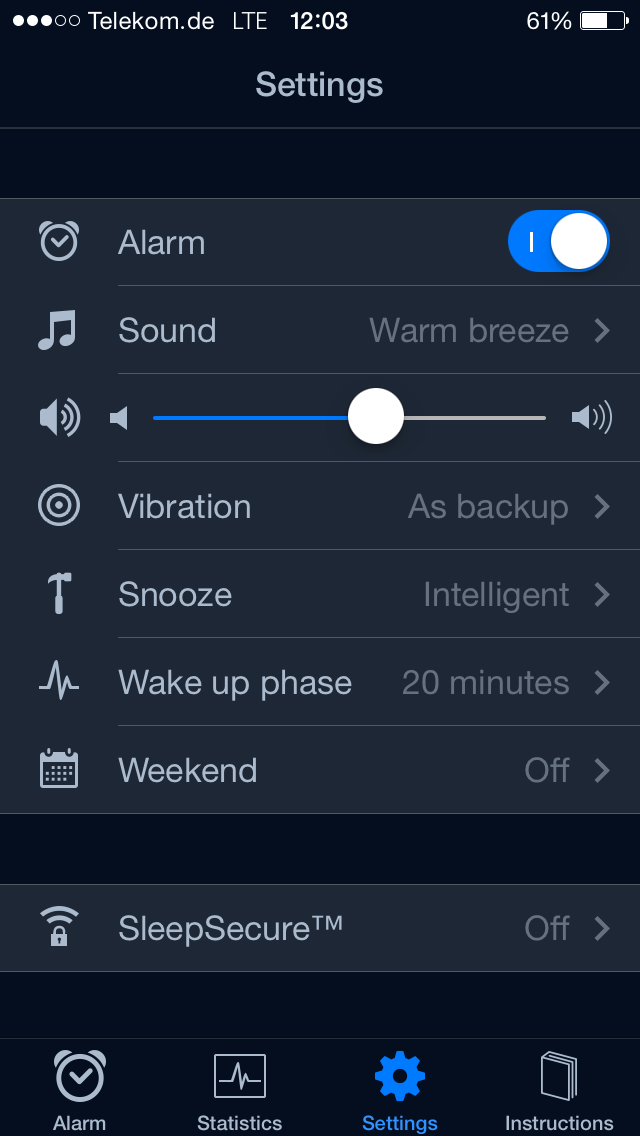
\includegraphics[scale=0.3]{images/SleepCycle/Settings1}  
    \caption{Sleep Cycle Settings}
    \label{fig:SCSettings}
  \end{minipage}
\end{figure}

Die weiteren Analyse-Grafiken zeigen beispielsweise welche Auswirkung unterschiedliche Tagesverläufe auf die Schlafqualität haben. 
Eine Grafik (Abb. \ref{fig:SCSleepNoteToday}) lässt den Nutzer Informationen über deren Schlaf sowie mögliche Ursachen für Störung der Schlafqualität betrachten.
Eine andere gibt Aufschluss über die durchschnittliche Schlafqualität anhand des Wochentages.

\begin{figure}[]
	\centering
    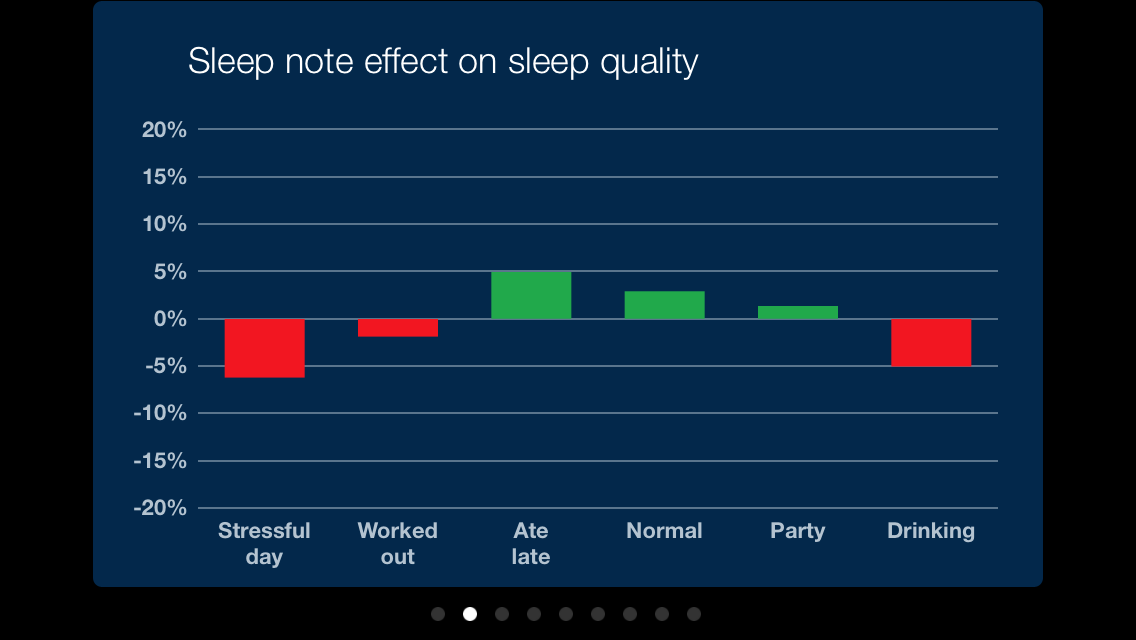
\includegraphics[scale=0.5]{images/SleepCycle/SleepNoteEffectOnSleepQuality} 
    \caption{Sleep Cycle Sleep note effect}
    \label{fig:SCDetail}
\end{figure}

\begin{figure}[]
    \centering
    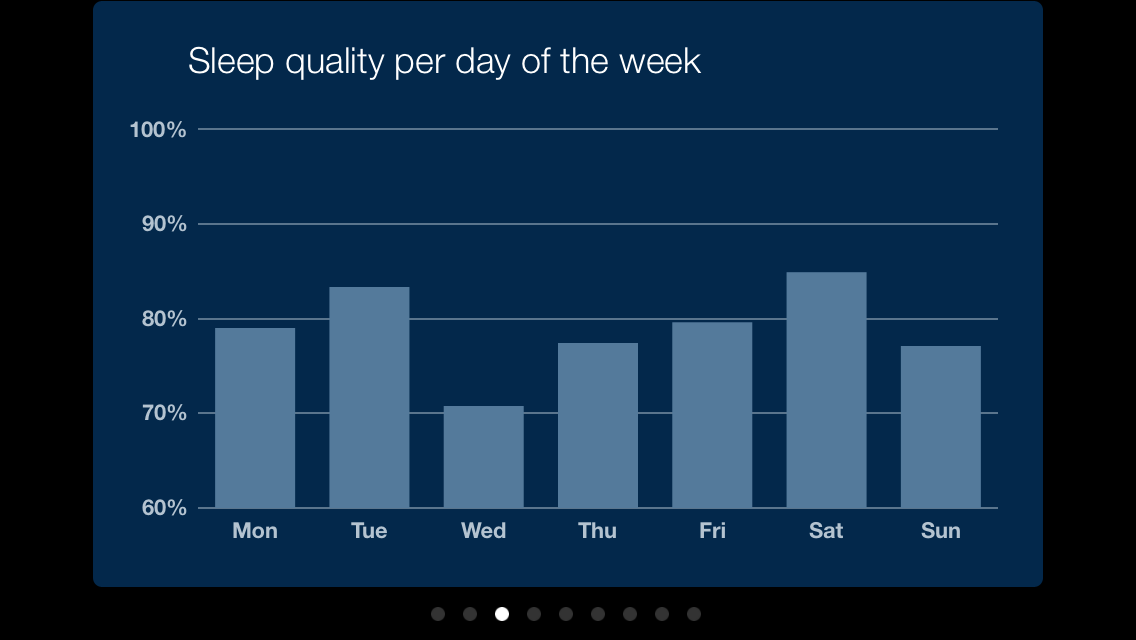
\includegraphics[scale=0.5]{images/SleepCycle/SleepQualityPerDayOfWeek}  
    \caption{Sleep Cycle Sleep quality per day of week}
    \label{fig:SCSettings}
\end{figure}

Mit Hilfe der Wochentagesanalyse lassen sich Einflüsse auf den Schlaf mit weiteren QS Tools, wie den innerhalb des Projektes benutzten Apps \textbf{Moves} \ref{ch:Apps:sec:Moves} und \textbf{Hueman} \ref{ch:Apps:sec:Hueman}, verknüpfen und auswerten.


%%% Local Variables: 
%%% mode: latex
%%% TeX-master: "thesis"
%%% End: 
